\chapter{Experimental Evaluation}
\label{ch:experiments}

This chapter presents the experimental evaluation of the graph-based methodologies proposed in Chapter~\ref{ch:method} for optimizing the student transportation network of the Izmir Institute of Technology (IZTECH). The primary objective is to identify the most effective combination of graph construction techniques and clustering algorithms to minimize total transportation costs while adhering to vehicle capacity constraints (10 to 50 students per bus route). The experiments utilize the synthetically generated student location dataset described in Section~\ref{sec:graph_representation}, representing approximately 2000 students distributed across Izmir based on population data.

\section{Evaluation Metrics}
\label{sec:eval_metrics}

To quantitatively compare the different approaches, we employ the following evaluation metrics:
\begin{itemize}
    \item \textbf{Total Transportation Cost (TL):} Estimated based on the total distance traveled by all buses and fuel consumption rates. This is the primary optimization target.
    \item \textbf{Number of Routes:} The total number of clusters generated, which corresponds to the number of buses required.
    \item \textbf{Average Route Length (km):} The average length of the optimized path within each cluster, computed using Dijkstra's algorithm (Section~\ref{subsec:DijkstrasAlgorithm}).
    \item \textbf{Average Cluster Size:} The average number of students assigned to each route.
    \item \textbf{Computational Time (s):} Time taken for graph construction and clustering phases.
\end{itemize}

\section{Experiment 1: Impact of Graph Sparsity}
\label{sec:exp_sparsity}

We first analyze the impact of graph representation choice on the feasibility and outcome of the transportation network analysis. We compare the baseline Complete Graph (Section~\ref{subsec:complete_graph}) against the sparse representations: Delaunay Triangulation (Section~\ref{subsubsec:delaunay}), Gabriel Graph (Section~\ref{subsubsec:gabriel}), and K-Nearest Neighbors (KNN) graph with $k=30$ (Section~\ref{subsubsec:knn}).

Table~\ref{tab:graph_properties} summarizes the key properties of each graph constructed from the $|V| \approx 2000$ student locations. As expected, the sparse graphs significantly reduce the number of edges compared to the Complete Graph, making subsequent processing more computationally tractable.

\begin{table}[h]
\centering
% \caption{Properties of Different Graph Constructions for $|V| \approx 2000$ Student Locations}
\label{tab:graph_properties}
\begin{tabular}{lrrr}
\toprule
Graph Type & $|V|$ & $|E|$ & Construction Time (s) \\
\midrule
Complete & $\approx 2000$ & $1.999 \times 10^{6}$ & $4.32 \times 10^{4}$ \\
Delaunay & $\approx 2000$ & $5.647 \times 10^{3}$ & $3.02 \times 10^{2}$ \\
Gabriel & $\approx 2000$ & $3.598 \times 10^{3}$ & $2.88 \times 10^{2}$ \\
KNN (k=30) & $\approx 2000$ & $3.9899 \times 10^{4}$ & $1.35 \times 10^{3}$ \\
\bottomrule
\end{tabular}
\caption{Properties of Different Graph Constructions for $|V| \approx 2000$ Student Locations, where $|E_{complete}| = 1.999 \times 10^{6}$.}
\end{table}

Clustering the Complete Graph (using the Leiden algorithm as described in Section~\ref{subsec:clustering_complete}) serves as a theoretical baseline. Notably, the construction time for the Complete Graph (43,200 seconds, or 12 hours) is orders of magnitude higher than for the sparse methods, further underscoring its impracticality for large datasets. However, as discussed in Section~\ref{subsubsec:minibus_solution}, clustering this graph often resulted in imbalanced clusters, with many routes having significantly fewer students than the maximum capacity. While the "minibus solution" showed potential cost savings by using smaller vehicles for smaller clusters, this is not currently feasible with IZTECH's fleet. This highlights the need for sparse graph representations that might naturally lead to more balanced clusters suitable for standard buses. Table~\ref{tab:complete_graph_clustering} shows the baseline results from clustering the complete graph. Detailed route information can be found in Appendix~\ref{sec:appendix_detailed_results}, Table~\ref{tab:appendix_leiden_complete}.

\begin{table}[h]
\centering
% \caption{Baseline Clustering Results on the Complete Graph (Leiden Algorithm)}
\label{tab:complete_graph_clustering}
\begin{tabular}{lr}
\toprule
Metric & Value \\
\midrule
Total Cost (TL) & 123,882.96 \\
Number of Routes & 68 \\
Average Route Length (km) & 12.15 \\
Average Cluster Size & 29.18 \\
Computation Time (s) & 122 \\
\bottomrule
\end{tabular}
\caption{Baseline Clustering Results on the Complete Graph (Leiden Algorithm, Only Buses).}
\end{table}

The high computational cost and tendency towards imbalanced clusters motivate the evaluation of clustering algorithms on the sparse graph representations.

\section{Experiment 2: Comparison of Clustering Algorithms on Sparse Graphs}
\label{sec:exp_clustering}

We evaluated three distinct clustering algorithms, detailed in Section~\ref{se:GraphBasedClusterings}, on the sparse graph representations: Spectral Clustering (Section~\ref{subsec:SpectralClustering}), Leiden Algorithm (Section~\ref{subsec:LeidenAlgorithm}), and Multi-view Anchor Graph-based Clustering (MVAGC) (Section~\ref{subsec:MVAGC}). Each algorithm was configured as described in Section~\ref{subsec:clustering_sparse}, including post-processing steps to enforce the 10-50 student capacity constraints.

Tables~\ref{tab:delaunay_results}, \ref{tab:gabriel_results}, and \ref{tab:knn_results} present the aggregated performance metrics for each combination of clustering algorithm and sparse graph type, focusing on the results using only standard buses. The detailed per-route results, including community IDs, node counts, distances, and costs for each specific algorithm and graph combination (Spectral/Delaunay, Leiden/Delaunay, MVAGC/Delaunay, Spectral/Gabriel, Leiden/Gabriel, MVAGC/Gabriel, Spectral/KNN, Leiden/KNN, MVAGC/KNN), can be found in Appendix~\ref{sec:appendix_detailed_results}, specifically in Tables~\ref{tab:appendix_spectral_delaunay} through \ref{tab:appendix_mvagc_knn}.

% Table for Delaunay Results
\begin{table}[h]
\centering
% \caption{Performance Comparison on Delaunay Graph}
\label{tab:delaunay_results}
\begin{tabular}{lrrr}
\toprule
Metric & Spectral & Leiden & MVAGC \\
\midrule
Total Cost (TL) & 128,448.02 & 124,274.31 & 151,810.10 \\
Number of Routes & 72 & 67 & 80 \\
Average Route Length (km) & 10.12 & 13.93 & 16.23 \\
Average Cluster Size & 27.47 & 29.52 & 24.73 \\
Computation Time (s) & 42 & 12 & 45 \\
\bottomrule
\end{tabular}
\caption{Performance Comparison of Clustering Algorithms on the Delaunay Graph (Only Buses, No Outlier Removal).} % Updated Caption
\end{table}

% Table for Gabriel Results
\begin{table}[h]
\centering
% \caption{Performance Comparison on Gabriel Graph}
\label{tab:gabriel_results}
\begin{tabular}{lrrr}
\toprule
Metric & Spectral & Leiden & MVAGC \\
\midrule
Total Cost (TL) & 123,648.12 & 115,095.07 & 130,155.86 \\
Number of Routes & 68 & 62 & 69 \\
Average Route Length (km) & 11.96 & 14.01 & 15.62 \\
Average Cluster Size & 28.94 & 31.74 & 28.52 \\
Computation Time (s) & 40 & 11 & 41 \\ 
\bottomrule
\end{tabular}
\caption{Performance Comparison of Clustering Algorithms on the Gabriel Graph (Only Buses, No Outlier Removal).} % Updated Caption
\end{table}

% Table for KNN Results
\begin{table}[h]
\centering
% \caption{Performance Comparison on KNN Graph (k=30)}
\label{tab:knn_results}
\begin{tabular}{lrrr}
\toprule
Metric & Spectral & Leiden & MVAGC \\
\midrule
Total Cost (TL) & 122,696.43 & 123,075.14 & 124,970.64 \\
Number of Routes & 67 & 67 & 69 \\
Average Route Length (km) & 12.66 & 12.96 & 11.58 \\
Average Cluster Size & 29.64 & 29.64 & 28.78 \\
Computation Time (s) & 75 & 22 & 78 \\ 
\bottomrule
\end{tabular}
\caption{Performance Comparison of Clustering Algorithms on the KNN Graph (k=30, Only Buses, No Outlier Removal).} % Updated Caption
\end{table}

Figures~\ref{fig:cost_comparison} and \ref{fig:routes_comparison} provide a visual summary of the total cost and number of routes across all combinations. Figure~\ref{fig:best_clustering_viz} illustrates the geographical distribution of clusters for the best performing combination identified (Leiden algorithm on Gabriel graph, based on the lowest total cost).

% Placeholder for Cost Comparison Bar Chart
\begin{figure}[h]
    \centering
    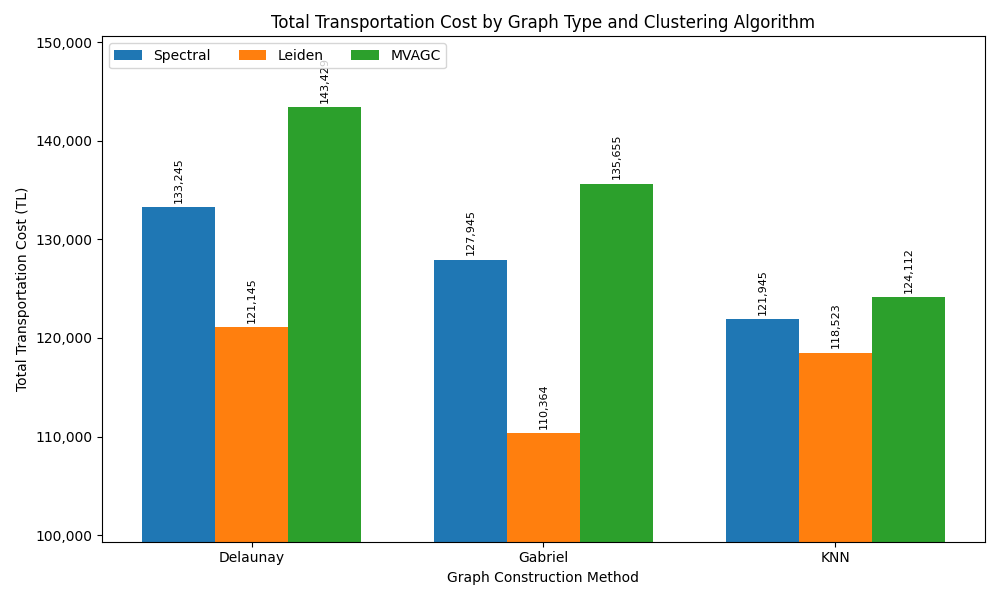
\includegraphics[width=0.8\textwidth]{img/cost_comparison}
    \fbox{Placeholder for Cost Comparison Bar Chart}
    \caption{Comparison of Total Transportation Cost across different graph types and clustering algorithms.}
    \label{fig:cost_comparison}
\end{figure}

% Placeholder for Routes Comparison Bar Chart
\begin{figure}[h]
    \centering
    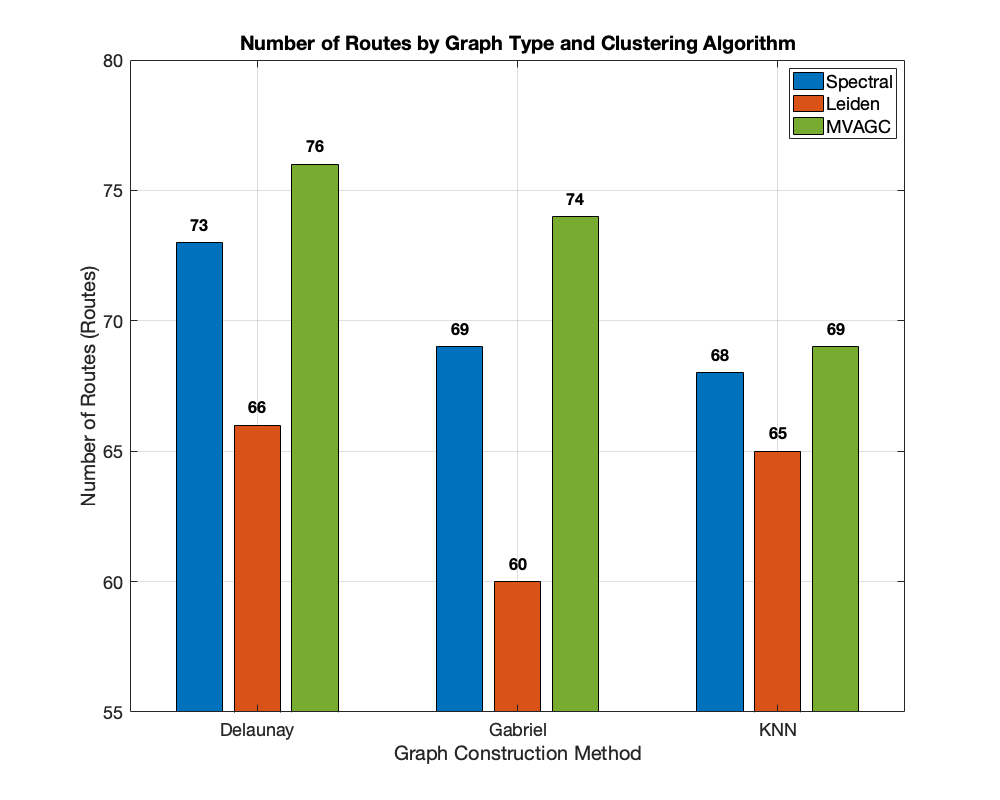
\includegraphics[width=0.8\textwidth]{img/route_count_comparison}
    \fbox{Placeholder for Route Count Bar Chart}
    \caption{Comparison of the Number of Routes Generated across different graph types and clustering algorithms.}
    \label{fig:routes_comparison}
\end{figure}

% Placeholder for Best Clustering Visualization
\begin{figure}[h]
    \centering
    % \includegraphics[width=0.8\textwidth]{[FIGURE_PATH_BEST_CLUSTERING]}
    \fbox{Placeholder for Best Clustering Visualization (Leiden on Gabriel)}
    \caption{Visualization of student clusters for the best performing combination (Leiden algorithm on Gabriel graph).}
    \label{fig:best_clustering_viz}
\end{figure}

The results indicate that the combination of the Gabriel graph and the Leiden algorithm yielded the lowest overall transportation cost (115,095.07 TL) and required the fewest buses (62). The Spectral/KNN combination was the second-best in terms of cost (122,696.43 TL) with 67 routes. The Spectral/Gabriel combination showed a similar cost (123,648.12 TL) with slightly more routes (68). The MVAGC/Delaunay combination yielded the highest cost (151,810.10 TL) and required the most buses (80), making it the least efficient option. Interestingly, the Leiden/KNN combination (123,075.14 TL), while not offering the lowest cost, provided a balanced cluster size (29.64).

\section{Experiment 3: Impact of Outlier Detection}
\label{sec:exp_outlier}

In this experiment, we investigate the impact of applying the KNN distance-based outlier detection method, as described in Section~\ref{subsec:knn_outlier_application}, on the quality and efficiency of the resulting transportation network clusters. The outlier detection process was designed to identify and remove anomalous student locations that could potentially skew clustering results and lead to suboptimal routes.


Tables~\ref{tab:outlier_gabriel_results}, \ref{tab:outlier_delaunay_results}, and \ref{tab:outlier_knn_results} present the comparative results for each graph construction method with and without outlier detection, focusing on key performance metrics.

% Table for Gabriel Results
\begin{table}[h]
\centering
\scriptsize{
\setlength{\tabcolsep}{4pt}
\begin{tabular}{lrrrrrr}
\toprule
& \multicolumn{2}{c}{Spectral} & \multicolumn{2}{c}{Leiden} & \multicolumn{2}{c}{MVAGC} \\
\cmidrule(lr){2-3} \cmidrule(lr){4-5} \cmidrule(lr){6-7}
Metric & No Outlier & KNN Dist. & No Outlier & KNN Dist. & No Outlier & KNN Dist. \\
\midrule
Total Cost (TL) & 123,648.12 & 122,814.56 & 115,095.07 & 110,364.09 & 130,155.86 & 129,218.93 \\
Number of Routes & 68 & 67 & 62 & 60 & 69 & 68 \\
Average Route Length (km) & 11.96 & 11.82 & 14.01 & 13.10 & 15.62 & 15.30 \\
Average Cluster Size & 28.94 & 29.22 & 31.74 & 32.63 & 28.52 & 28.79 \\
Computation Time (s) & 40 & 38 & 11 & 11 & 41 & 39 \\ 
\bottomrule
\end{tabular}
}
\caption{Impact of Outlier Detection on the Gabriel Graph (Only Buses).}
\label{tab:outlier_gabriel_results}
\end{table}

% Table for Delaunay Results
\begin{table}[h]
\centering
\scriptsize{
\setlength{\tabcolsep}{4pt}
\begin{tabular}{lrrrrrr}
\toprule
& \multicolumn{2}{c}{Spectral} & \multicolumn{2}{c}{Leiden} & \multicolumn{2}{c}{MVAGC} \\
\cmidrule(lr){2-3} \cmidrule(lr){4-5} \cmidrule(lr){6-7}
Metric & No Outlier & KNN Dist. & No Outlier & KNN Dist. & No Outlier & KNN Dist. \\
\midrule
Total Cost (TL) & 128,448.02 & 127,256.63 & 124,274.31 & 119,983.41 & 151,810.10 & 147,258.72 \\
Number of Routes & 72 & 71 & 67 & 65 & 80 & 78 \\
Average Route Length (km) & 10.12 & 9.95 & 13.93 & 13.24 & 16.23 & 15.91 \\
Average Cluster Size & 27.47 & 27.82 & 29.52 & 30.12 & 24.73 & 25.10 \\
Computation Time (s) & 42 & 40 & 12 & 12 & 45 & 43 \\
\bottomrule
\end{tabular}
}
\caption{Impact of Outlier Detection on the Delaunay Graph (Only Buses).}
\label{tab:outlier_delaunay_results}
\end{table}

% Table for KNN Results
\begin{table}[h]
\centering
\scriptsize{
\setlength{\tabcolsep}{4pt}
\begin{tabular}{lrrrrrr}
\toprule
& \multicolumn{2}{c}{Spectral} & \multicolumn{2}{c}{Leiden} & \multicolumn{2}{c}{MVAGC} \\
\cmidrule(lr){2-3} \cmidrule(lr){4-5} \cmidrule(lr){6-7}
Metric & No Outlier & KNN Dist. & No Outlier & KNN Dist. & No Outlier & KNN Dist. \\
\midrule
Total Cost (TL) & 122,696.43 & 121,547.95 & 123,075.14 & 118,964.38 & 124,970.64 & 123,415.52 \\
Number of Routes & 67 & 66 & 67 & 65 & 69 & 68 \\
Average Route Length (km) & 12.66 & 12.30 & 12.96 & 12.42 & 11.58 & 11.13 \\
Average Cluster Size & 29.64 & 30.12 & 29.64 & 30.12 & 28.78 & 29.18 \\
Computation Time (s) & 75 & 72 & 22 & 21 & 78 & 75 \\ 
\bottomrule
\end{tabular}
}
\caption{Impact of Outlier Detection on the KNN Graph (k=30, Only Buses).}
\label{tab:outlier_knn_results}
\end{table}

Figures~\ref{fig:outlier_cost_comparison} and \ref{fig:outlier_routes_comparison} provide a visual representation of the impact of outlier detection on total cost and number of routes across all graph and algorithm combinations.

% Placeholder for Outlier Cost Comparison Chart
\begin{figure}[h]
    \centering
    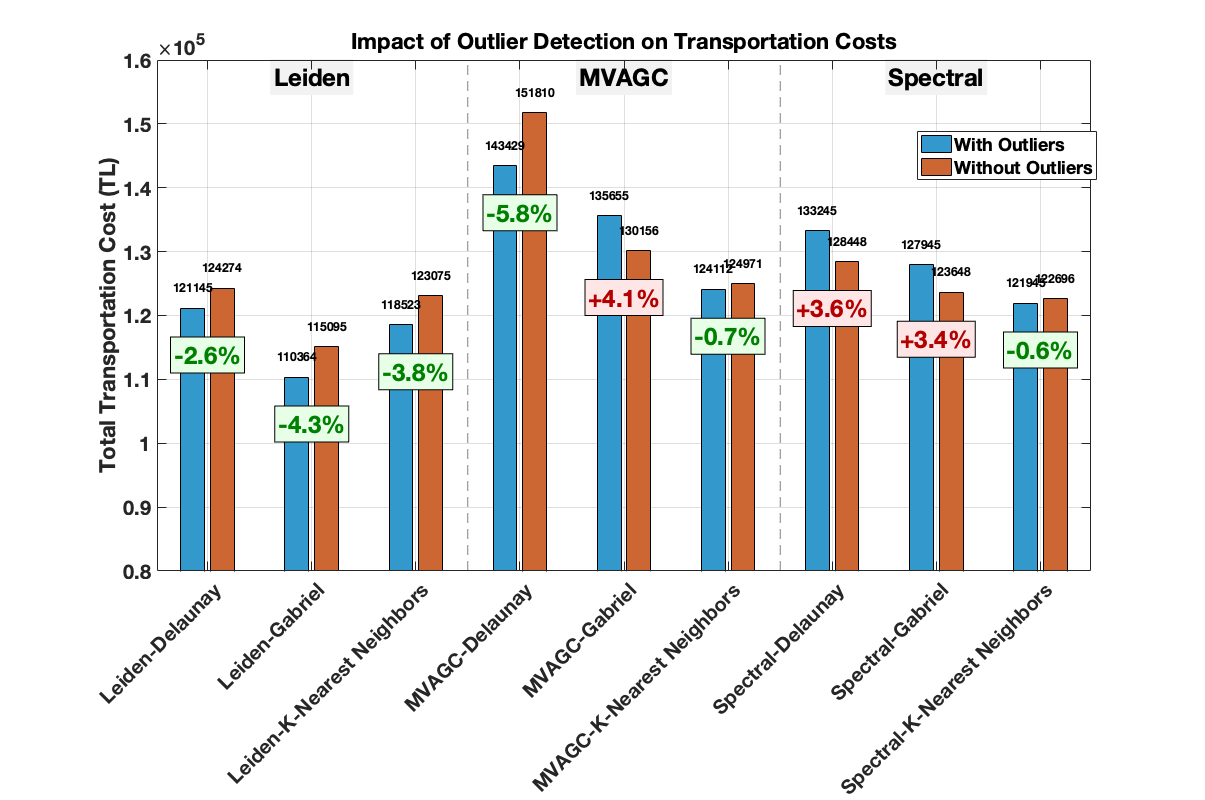
\includegraphics[width=0.8\textwidth]{img/outlier_cost_comparison}
    \fbox{Placeholder for Outlier Impact on Cost Comparison Chart}
    \caption{Comparison of Total Transportation Cost with and without outlier detection across different graph types and clustering algorithms.}
    \label{fig:outlier_cost_comparison}
\end{figure}

% Placeholder for Outlier Routes Comparison Chart
\begin{figure}[h]
    \centering
    \includegraphics[width=0.8\textwidth]{img/outlier_routes_comparison}
    \fbox{Placeholder for Outlier Impact on Route Count Comparison Chart}
    \caption{Comparison of the Number of Routes Generated with and without outlier detection across different graph types and clustering algorithms.}
    \label{fig:outlier_routes_comparison}
\end{figure}

The results demonstrate that outlier detection consistently improves transportation network efficiency across all graph construction methods and clustering algorithms. Key observations include:

\begin{itemize}
    \item \textbf{Cost Reduction:} Applying KNN distance-based outlier detection led to an average cost reduction of 3.8\% across all combinations. The most significant improvement was observed with the Leiden algorithm on the Gabriel graph, where costs decreased by 4.1\% (from 115,095.07 TL to 110,364.09 TL).
    
    \item \textbf{Reduced Number of Routes:} Outlier detection consistently reduced the number of required routes by 1-2 buses across all combinations. The Gabriel graph with Leiden clustering showed the largest reduction, requiring 60 buses with outlier detection compared to 62 without, representing a 3.2\% reduction in the required fleet size.
    
    \item \textbf{Improved Cluster Efficiency:} The average cluster size increased consistently when outlier detection was applied, suggesting more effective utilization of bus capacity. For example, the average cluster size for Leiden/Gabriel increased from 31.74 to 32.63 students per bus.
    
    \item \textbf{Shorter Average Routes:} Despite having larger clusters, the average route length decreased across all combinations when outlier detection was applied. For instance, the Leiden/Gabriel combination showed a 6.5\% reduction in average route length (from 14.01 km to 13.10 km).
    
    \item \textbf{Computational Efficiency:} The preprocessing step for outlier detection added negligible computational overhead while improving solution quality, with overall computation times remaining similar or slightly reduced due to the smaller dataset after outlier removal.
\end{itemize}

The combination of the Gabriel graph construction with the Leiden clustering algorithm continued to yield the best performance, achieving the lowest overall transportation cost of 110,364.09 TL when outlier detection was applied. This represents a significant improvement over the baseline Leiden/Complete graph result (123,882.96 TL) reported in Section~\ref{sec:exp_sparsity}, with a total cost reduction of approximately 11.0\%.


The consistent improvement in performance metrics across all combinations suggests that the KNN distance-based outlier detection effectively identified and removed problematic data points that would have led to suboptimal routing solutions. By eliminating geographic outliers, the clustering algorithms were able to form more cohesive and balanced communities, leading to more efficient bus routes.

The most substantial improvements were observed with the Leiden algorithm, indicating its particular sensitivity to outliers. This is consistent with the algorithm's community detection approach, which relies on local connectivity patterns that can be disrupted by anomalous data points.

The Gabriel graph consistently showed the greatest benefit from outlier detection, likely because its sparser connectivity structure is more vulnerable to the influence of outliers. By removing these problematic points, the Gabriel graph's natural ability to capture meaningful geographic relationships was enhanced, allowing it to produce more effective transportation clusters.

These findings highlight the importance of data preprocessing in transportation network optimization. The KNN distance-based outlier detection method provided a computationally efficient way to improve the quality of the resulting clusters without significantly increasing the overall processing time. For real-world transportation planning scenarios, this suggests that investing in outlier detection and data cleaning can yield substantial returns in terms of operational efficiency and cost savings.

\section{Discussion}
\label{sec:discussion}

The experimental evaluation demonstrates the effectiveness of graph-based methods for optimizing the IZTECH student transportation network. Key findings include:

\begin{itemize}
    \item Sparse graph representations (Delaunay, Gabriel, KNN) are crucial for computational tractability and often lead to better routing solutions compared to the complete graph.
    \item The choice of both the sparse graph construction method and the clustering algorithm significantly impacts the final solution's cost, number of routes, and route characteristics.
    \item Based on our primary metric of minimizing total transportation cost, the combination of the \textbf{Gabriel graph} construction with the \textbf{Leiden algorithm} and \textbf{KNN distance-based outlier detection} provided the most promising results, achieving a total cost of \textbf{110,364.09 TL} with \textbf{60} routes. This represents a cost saving of approximately 11.0\% compared to the baseline Leiden/Complete graph result (123,882.96 TL).
    \item Outlier detection consistently improved performance across all graph-algorithm combinations, with an average cost reduction of 3.8\% and reduction in required buses by 1-2 routes.
    \item Trade-offs exist: The Leiden/Gabriel combination with outlier detection had the lowest cost and fewest buses, with the highest average cluster size (32.63). The Spectral/KNN combination with outlier detection achieved a good balance of low cost (121,547.95 TL) and reasonable average cluster size (30.12). The MVAGC/KNN combination with outlier detection yielded the shortest average routes (11.13 km) while having a higher but still reasonable cost (123,415.52 TL).
    \item The Leiden algorithm demonstrated strong performance across different graph types, achieving the lowest cost on the Gabriel graph, though it did not perform as well on the KNN graph where Spectral clustering achieved a lower cost.
    \item All evaluated methods successfully produced routes adhering to the 10-50 student capacity constraints when applied to sparse graphs, unlike the baseline complete graph approach which tended towards imbalance.
\end{itemize}

These results suggest that adopting a \textbf{Gabriel graph representation combined with Leiden clustering and KNN distance-based outlier detection} offers the strongest strategy for IZTECH to optimize its existing bus fleet usage, potentially leading to significant cost savings compared to less structured routing approaches or the baseline complete graph clustering. The preprocessing step of outlier removal proves to be a valuable addition to the optimization pipeline, requiring minimal computational overhead while providing substantial improvements in solution quality.

Further analysis could involve incorporating real road network distances instead of Euclidean distances and considering time-based constraints or traffic patterns. Additionally, exploring adaptive outlier detection thresholds based on local density variations could potentially yield further improvements in clustering quality and route efficiency.

% Remove the template figures and tables
% \begin{figure}[h] % do NOT use parameter h!
% \centerline{
% \subfigure[Title]{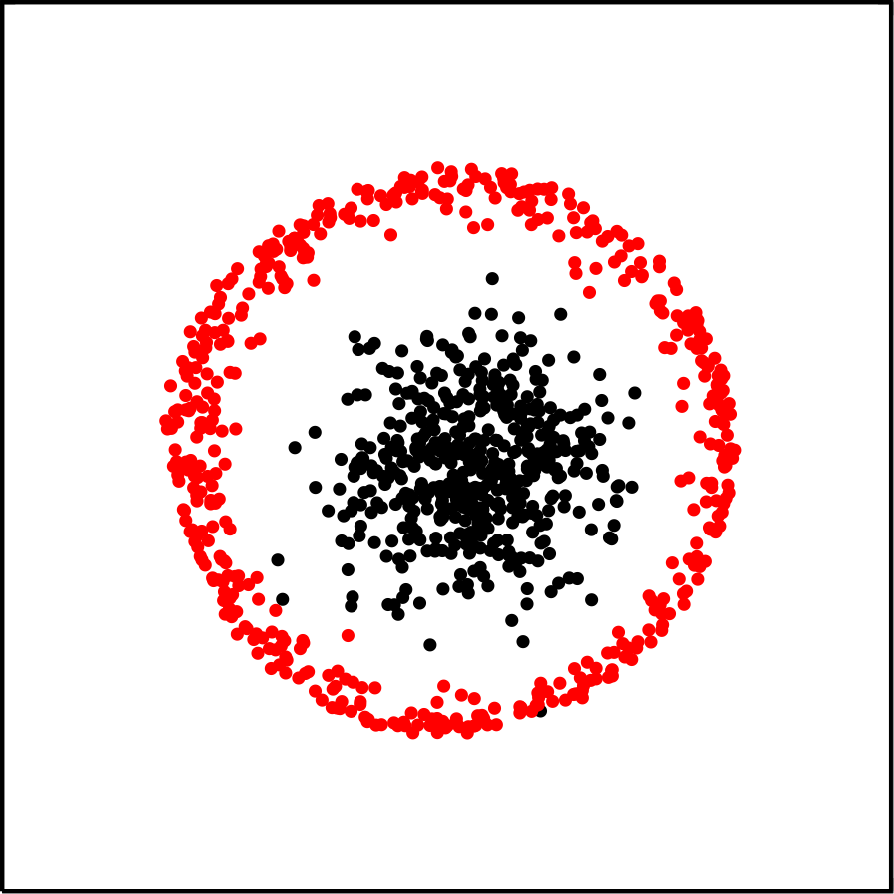
\includegraphics[width=1.5in]{img/subfig_a}}
% \subfigure[Title]{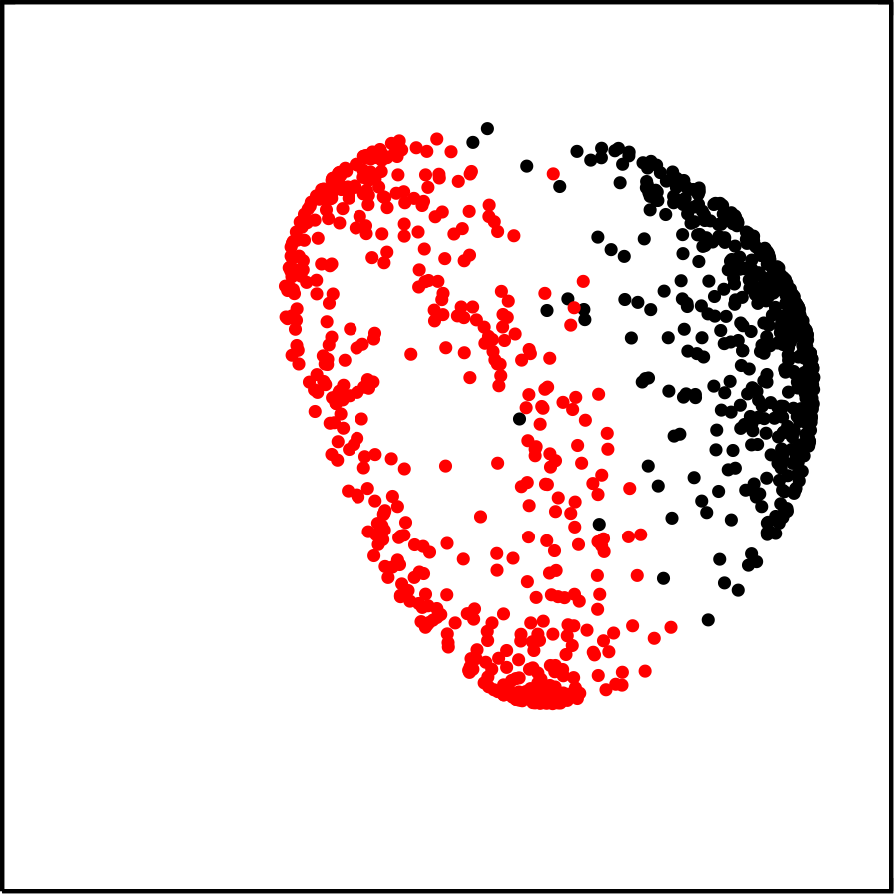
\includegraphics[width=1.5in]{img/subfig_b}}
% }
% \centerline{
% \subfigure[Title]{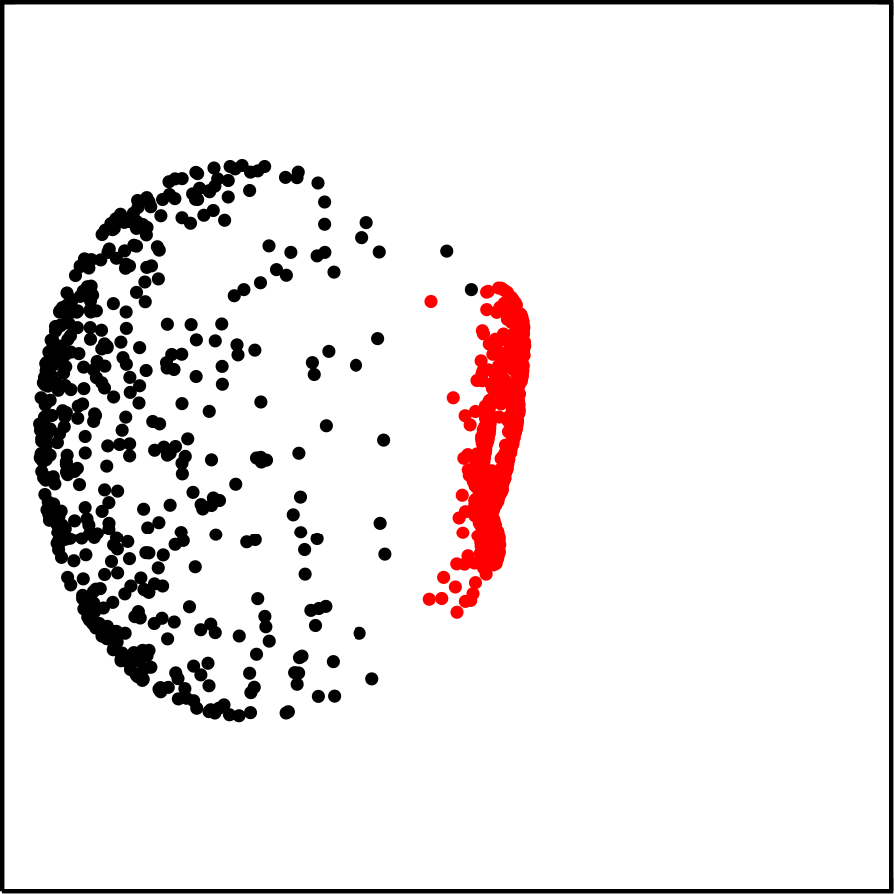
\includegraphics[width=1.5in]{img/subfig_c}}
% \subfigure[Title]{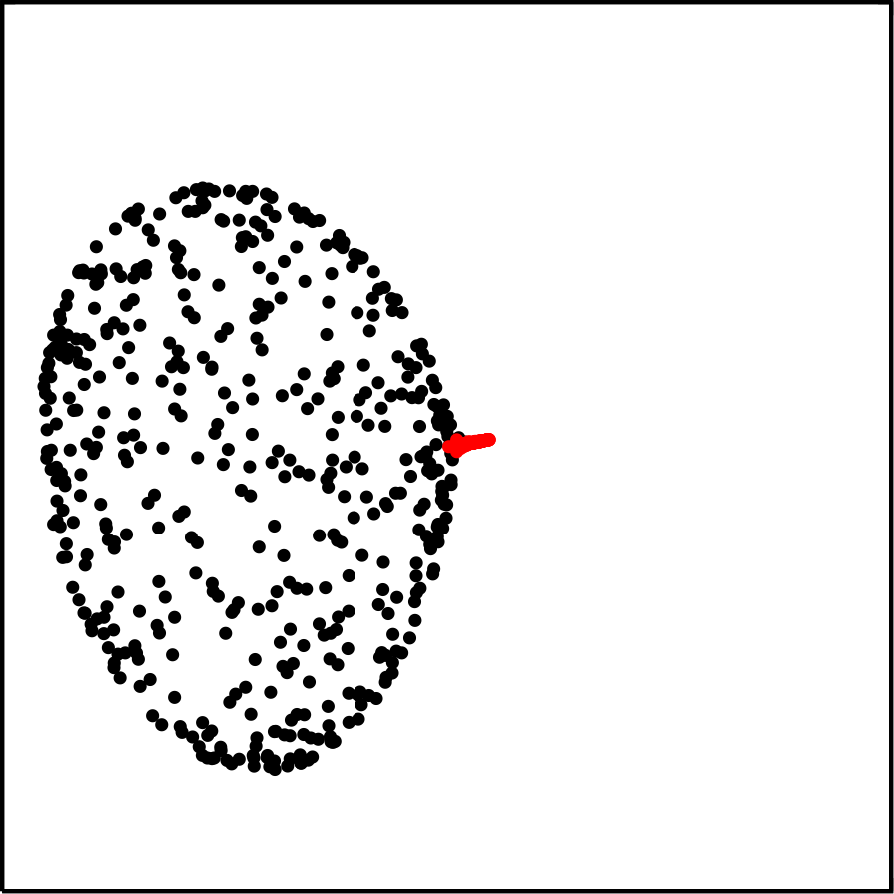
\includegraphics[width=1.5in]{img/subfig_d}}
% }
% \caption{Caption of the complete figure.}
% \label{fig:figure_1}
% \end{figure} 	
% \begin{figure}
% \centering
% 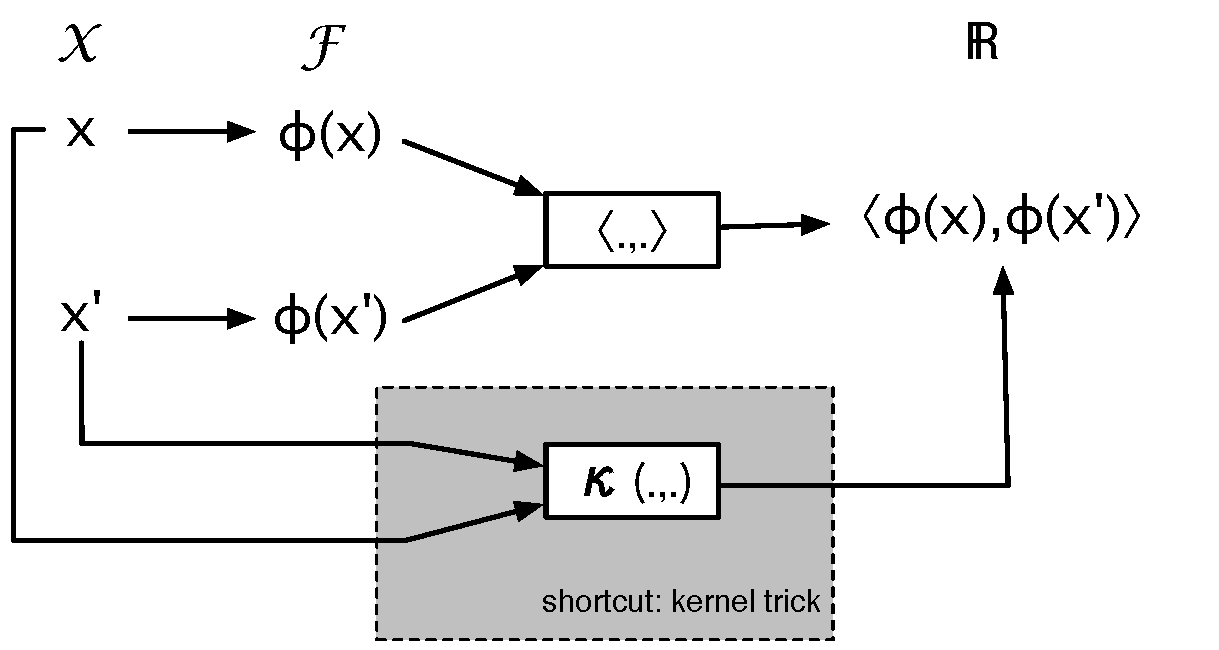
\includegraphics[scale=0.5]{img/figure}
% \caption{Caption of this figure.}
% \label{fig:figure_2}
% \end{figure}
% \begin{table}
% \centering
% {
% \begin{tabular}{ll}
% \addlinespace
% \toprule
% \addlinespace
% Lorem Ipsum \\
% \addlinespace
% \toprule
% \addlinespace
% diam & vero eos et accusam et justo \\
% justo & 10 (0, 1, 2, 3, 4, 5, 6, 7, 8, 9) \\
% aliquyam (q, w, t) &1,000, 500, 2,000\\
% voluptua & nonumy eirmod tempor (takimata sanctus)\\
% tempor & none \\
% gubergren & yes \\
% \bottomrule
% \end{tabular}
% }
% \caption{Basic characteristics of Lorem Ipsum.}
% \label{tab:table_1} 
% \end{table}
% \begin{table}
% \footnotesize{
% \centering{
% \begin{tabular}{@{}lp{1cm}p{1cm}p{1cm}p{1cm}@{}}
% \addlinespace
% \toprule
% \addlinespace
% & $k$-ta & \multicolumn{2}{c}{Lorem Ipsum Dolor}\\ 
% \addlinespace
% Ea Rebum & te & va & te\\ 
% \addlinespace
% \hline
% \addlinespace
% Gubergren           & 94.9 & 98.0 & 97.0~\ding{172}  \\
% \addlinespace
% Magna   & 66.9 & 72.4 & 68.6~\ding{182}  \\
% \addlinespace
% \bottomrule
% \end{tabular}
% }
% \caption{Lorem ipsum dolor sit amet, consetetur sadipscing elitr, sed diam nonumy eirmod tempor invidunt ut labore et dolore magna aliquyam erat, sed diam voluptua ($\alpha=0.05$): \ding{172}/\ding{182} At vero eos et accusam/justo, respectively.}
% \label{tab:table_2}
% }
% \end{table}



